\section{Cahier des charges}

	Cette section a pour rôle de présenter le cahier des charges de ce projet. Nous introduisons également le concept de générateur de contenu statique. La seconde partie de cette section liste quelques cas d'utilisation afin d'illustrer le fonctionnement souhaité par ce projet. Notez que les fonctionnalités en elles-même seront détaillées dans la Section 4.\\
	
	Le cahier des charges de ce projet est volontairement resté assez flou. En effet, les seules consignes données sont de concevoir un générateur de contenu statique qui donne à l'utilisateur une grande souplesse d'utilisation afin de pouvoirs effectuer des tâches diverses. Ce générateur de contenu statique doit aussi être simple à utiliser pour le "grand public" et ne doit donc pas faire appel à des connaissances en programmation. Afin de préciser ce que sont les "tâches diverses" que ce générateur doit être capable d'accomplir, quelques cas d'utilisations sont illustrés dans cette section.\\
	
	
	\subsection{Générateur de contenu statique}
	%todo insister sur le rôle, pas un générateur de site web, différence avec CMS ? Motivation générale du projet
		Nous introduisons ici les notations que nous allons utiliser tout au long de ce rapport. Cette sous-section contient également notre définition d'un générateur de contenu statique. 
	
		\begin{defn}
			Un \textbf{générateur de contenu} sert à lier des données à un \textit{template} (ou gabarit) afin de générer du contenu (document, site web, ...). Il sera qualifié de \textbf{statique} si ce contenu est identique peu importe le contexte dans lequel il est consulté. Les données, les \textit{templates} et les contenus sont appelés \textbf{paramètres} d'un générateur de contenu statique dans le reste de ce rapport.
		\end{defn}
		
		\begin{defn}
			Un \textbf{item} est la brique de base d'un paramètre. Il s'agit d'une abstraction de ce qu'un paramètre représente comme valeur. En pratique un \textit{item} peut être une page web, un fichier texte, une base de données, une structure de données, ...
		\end{defn}
		
		\begin{defn}
			 La \textbf{multiplicité} des paramètres d'un générateur de contenu statique est le nombre d'\textit{items} qu'ils représentent.
		\end{defn}
		
		\begin{note}
			Nous utilisons parfois les termes "générateur de contenu statique" et "générateur" de manière interchangeable afin d'éviter les répétitions et les lourdeurs d'écritures.
		\end{note}
		
		 A savoir que les générateurs de contenu statique sont très utilisés pour produire des sites web statiques. De ce cas, les \textit{CMS} (ou SGC) peuvent être considérés comme des générateurs de contenu statique. Ils offrent toutefois plus de fonctionnalités qu'un générateur classique mais cela s'écarte du cadre de ce projet. Cela n'est vrai que pour les \textit{CMS} qui ne génère que du contenu statique.\\
		 
		 Notre générateur de contenu statique a une vocation un peu plus générale car il permettra de générer à peu près n'importe quel type de contenu statique. Leur utilisation est souvent liée au concept de \textit{templates} qui permettent de séparer les informations de la mise en page en elle-même. La Figure \ref{fig:use_of_generator} montre une utilisation type de ce genre de générateur. L'Exemple \ref{exmpl:GDCS} illustre cela grâce à un cas simple et concret.\\
		
		\begin{figure}[h]
			\begin{center}
				\begin{tikzpicture}
				\coordinate (Data) at (-3, 0);
				\coordinate (Template) at (-1, 1);
				\coordinate (Content) at (2, 0);
				\coordinate (Center) at (-1, 0);
				
				\draw (-4, 0) circle (1) ;
				\draw (-4, 0) node{$\text{Données}$};
				\draw[>=latex, ->] (Data) -- (Center);
				
				\draw[rounded corners]  (2, -1) rectangle(4, 1);
				\draw (3, 0) node{$\text{Contenu}$};
				\draw[>=latex, ->] (Center) --(Content);
				
				\draw(-2, 1) rectangle(0, 3);
				\draw (-1, 2) node{$\text{Template}$};
				\draw[>=latex, ->]  (Template) -- (Center);
			\end{tikzpicture}
			\caption{Utilisation type d'un générateur de contenu statique}
			\label{fig:use_of_generator}
			\end{center}
		\end{figure}
		
		\begin{exmpl}
			\label{exmpl:GDCS}
			Les Figures \ref{exmpl:GDCS:data}, \ref{exmpl:GDCS:template}, \ref{exmpl:GDCS:content} représentent respectivement les données à utiliser, le \textit{template} à appliquer et le contenu ainsi généré. Nous pouvons ainsi constater que le générateur de contenu statique génère ce dernier en remplaçant les champs du \textit{template} par les valeurs contenues dans le fichier de données.
			\begin{figure}[!]
				\centering
				\lstinputlisting[inputencoding=utf8/latin1]{codeSample/example/players.json}
				\caption{Données au format JSON}
				\label{exmpl:GDCS:data}
			\end{figure}				
			\begin{figure}[!]
				\centering
				\lstinputlisting[inputencoding=utf8/latin1]{codeSample/example/template.j2}
				\caption{Template au format Jinja2}
				\label{exmpl:GDCS:template}
			\end{figure}%
			\begin{figure}[!]
				\centering
				\lstinputlisting[inputencoding=utf8/latin1]{codeSample/example/players.txt}
				\caption{Contenu au format \textit{txt}}
				\label{exmpl:GDCS:content}
			\end{figure}			
			
		\end{exmpl}

	\subsection{Cas d'utilisations}
	
		Nous distinguons principalement trois cas d'utilisations propres aux générateurs de contenu statique. Nous appelons ces trois cas comme suit: \textit{OneToMany}, \textit{ManyToOne} et \textit{ManyToMany}. En pratique, ces trois cas se distinguent par la multiplicités des paramètres du générateur de contenu statique. Chacun d'entre eux est illustré à l'aide d'une figure explicitant leurs multiplicités.\\
		
		Nous présentons également 2 cas d'utilisations supplémentaires qui ne sont pas directement réalisables grâce à notre générateur de contenu statique. Nous présentons donc aussi des techniques pour contourner ces limitations. Ces cas d'utilisations sont appelés \textit{ManyTemplatesIn} et \textit{ManyTemplatesOut}.\\
		
		\subsubsection*{OneToMany}
		
			La cas \textit{OneToMany} désigne l'utilisation d'un générateur de contenu statique en vue de générer plusieurs \textit{items} de contenus à partir d'un seul \textit{item} de données. Ce cas d'utilisation est illustré par la Figure \ref{fig:OneToMany} en considérant que \textbf{n} est la multiplicité des contenus à générer. L'Exemple \ref{exmpl:OneToMany} met en pratique ce cas d'utilisation.
			
			\begin{figure}[!]
				\begin{center}
					\begin{tikzpicture}
					\coordinate (Data) at (-3, 0);
					\coordinate (Template) at (-1, 1);
					\coordinate (Content) at (2, 0);
					\coordinate (Center) at (-1, 0);
					
					\draw (-4, 0) circle (1) ;
					\draw (-4, 0) node{$\text{Données}$};
					\draw[>=latex, ->] (Data) -- (Center) node[near start, above] {$1$};
					
					\draw[rounded corners]  (2, -1) rectangle(4, 1);
					\draw (3, 0) node{$\text{Contenu}$};
					\draw[>=latex, ->] (Center) --(Content) node[near end, above] {$n$};
					
					\draw(-2, 1) rectangle(0, 3);
					\draw (-1, 2) node{$\text{Template}$};
					\draw[>=latex, ->]  (Template) -- (Center) node[midway, right]{1};
					\end{tikzpicture}
					\caption{Représentation du cas \textbf{OneToMany}.}
					\label{fig:OneToMany}
				\end{center}
			\end{figure}
			
			\begin{exmpl}
				\label{exmpl:OneToMany}
				 Par exemple, pour un site de vente, cela correspond à générer autant de page web qu'il y a de produits, chaque page ne contenant les caractéristiques que d'un unique produit (\textit{items} de contenu). L'\textit{item} de données est ici représenté par une base de données contenant les caractéristiques de tous les produits. Dans cet exemple, le \textit{template} est appliqué à chaque produit individuellement pour générer une page web par produit.
			\end{exmpl}
		
		\subsubsection*{ManyToOne}
		
			Le second cas, \textit{ManyToOne}, est le cas inverse de \textit{OneToMany}. En effet, ce cas désigne l'utilisation d'un générateur de contenu statique qui génère un seul \textit{item} à partir de plusieurs. Cela donne la Figure \ref{fig:ManyToOne} où \textbf{n} est la multiplicité des données. L'Exemple \ref{exmpl:ManyToOne} met ce cas d'utilisation en pratique.
			
			\begin{exmpl}
				\label{exmpl:ManyToOne}
				Par exemple, pour un blog, cela correspond à générer une page web contenant l'ensemble de tous les posts (\textit{item} de contenu). Celle-ci serait générée à partir d'un ensemble de fichier contenant chacun un post (\textit{items} de données). Dans ce cas, le \textit{template} est appliqué une  fois sur l'ensemble des posts dans le but de générer une unique page web.
			\end{exmpl}
		
			\begin{figure}[!]
				\begin{center}
					\begin{tikzpicture}
					\coordinate (Data) at (-3, 0);
					\coordinate (Template) at (-1, 1);
					\coordinate (Content) at (2, 0);
					\coordinate (Center) at (-1, 0);
					
					\draw (-4, 0) circle (1) ;
					\draw (-4, 0) node{$\text{Données}$};
					\draw[>=latex, ->] (Data) -- (Center) node[near start, above] {$n$};
					
					\draw[rounded corners]  (2, -1) rectangle(4, 1);
					\draw (3, 0) node{$\text{Contenu}$};
					\draw[>=latex, ->] (Center) --(Content) node[near end, above] {$1$};
					
					\draw(-2, 1) rectangle(0, 3);
					\draw (-1, 2) node{$\text{Template}$};
					\draw[>=latex, ->]  (Template) -- (Center) node[midway, right]{1};
					\end{tikzpicture}
					\caption{Représentation du cas \textbf{ManyToOne}.}
					\label{fig:ManyToOne}
				\end{center}
			\end{figure}
			
		\subsubsection*{ManyToMany}
			
			Le dernier cas est celui que nous appellerons \textit{ManyToMany}. Ce cas est en fait une généralisation des deux cas précédents. Effectivement, \textit{ManyToMany} désigne l'utilisation d'un générateur de contenu statique en vue de générer plusieurs \textit{items} de contenu à partir de plusieurs \textit{items} de données. La Figure \ref{fig:ManyToMany} permet une vision plus claire de ce cas où \textbf{n} désigne la multiplicité des données et \textbf{m} la multiplicité des contenus. L'Exemple \ref{exmpl:ManyToMany} met en pratique ce cas d'utilisation.\\
			
			\begin{exmpl}
				\label{exmpl:ManyToMany}
				 Par exemple, pour un blog, cela correspond à produire un certains nombres de pages web (disons 100 pages) listant les posts 10 par 10 (\textit{items} de contenus) grâce à un ensemble de fichiers contenant chacun un post (\textit{items} de données). Ici, le \textit{template} est appliqué 100 fois sur des ensembles de 10 posts jusqu'à ce que tous les posts soient traités. Cela génère les 100 pages contenant chacune 10 posts.  
			\end{exmpl}
			
			\begin{figure}[!]
				\begin{center}
					\begin{tikzpicture}
					\coordinate (Data) at (-3, 0);
					\coordinate (Template) at (-1, 1);
					\coordinate (Content) at (2, 0);
					\coordinate (Center) at (-1, 0);
					
					\draw (-4, 0) circle (1) ;
					\draw (-4, 0) node{$\text{Données}$};
					\draw[>=latex, ->] (Data) -- (Center) node[near start, above] {$n$};
					
					\draw[rounded corners]  (2, -1) rectangle(4, 1);
					\draw (3, 0) node{$\text{Contenu}$};
					\draw[>=latex, ->] (Center) --(Content) node[near end, above] {$m$};
					
					\draw(-2, 1) rectangle(0, 3);
					\draw (-1, 2) node{$\text{Template}$};
					\draw[>=latex, ->]  (Template) -- (Center) node[midway, right]{$1$};
					\end{tikzpicture}
					\caption{Représentation du cas \textbf{ManyToMany}.}
					\label{fig:ManyToMany}
				\end{center}
			\end{figure}
		
		%todo expliquer pourquoi ils sont réalisables sans implémentation
		
		\subsubsection*{ManyTemplatesIn}
		%todo cas théorique, expliquer en montrant un exemple
			Ce cas d'utilisation implique  d'utiliser un générateur de contenu statique dans le but de produire un fichier contenant plusieurs fois les mêmes données mais agencées par un \textit{template} différent. Nous n'avons pas trouvé d'exemple pratique pour illustrer ce cas mais la Figure \ref{fig:ManyTemplatesIn:out} permet de visualiser le format de fichier générer dans ce cas. La Figure \ref{fig:ManyTemplatesIn} exhibe plus clairement les multiplicités de ce cas, où \textbf{n} est le nombre de \textit{templates} à appliquer sur le fichier de données.
			
			\begin{figure}[!]
				\begin{center}
					\begin{tikzpicture}
					\coordinate (Data) at (-3, 0);
					\coordinate (Template) at (-1, 1);
					\coordinate (Content) at (2, 0);
					\coordinate (Center) at (-1, 0);
					
					\draw (-4, 0) circle (1) ;
					\draw (-4, 0) node{$\text{Données}$};
					\draw[>=latex, ->] (Data) -- (Center) node[near start, above] {$1$};
					
					\draw[rounded corners]  (2, -1) rectangle(4, 1);
					\draw (3, 0) node{$\text{Contenu}$};
					\draw[>=latex, ->] (Center) --(Content) node[near end, above] {$1$};
					
					\draw(-2, 1) rectangle(0, 3);
					\draw (-1, 2) node{$\text{Template}$};
					\draw[>=latex, ->]  (Template) -- (Center) node[midway, right]{$n$};
					\end{tikzpicture}
					\caption{Représentation du cas \textbf{ManyTemplatesIn}.}
					\label{fig:ManyTemplatesIn}
				\end{center}
			\end{figure}
			
			
			\begin{figure}[!]
				\begin{center}
					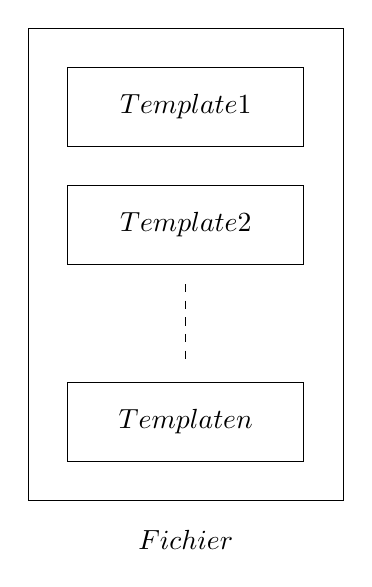
\begin{tikzpicture}
					\coordinate (Data) at (-3, 0);
					\coordinate (Template) at (-1, 1);
					\coordinate (Content) at (2, 0);
					\coordinate (Center) at (-1, 0);
				
					
					\draw(0, 0) rectangle(4, 6);
					\draw (2, -0.5) node{$\text{Fichier}$};
					
					\draw(0.5, 4.5) rectangle(3.5, 5.5);
					\draw (2, 5) node{$\text{Template 1}$};
					
					\draw(0.5, 3) rectangle(3.5, 4);
					\draw (2, 3.5) node{$\text{Template 2}$};
					
					\draw[dashed] (2, 2.75) -- (2, 1.75);
					
					\draw(0.5, 0.5) rectangle(3.5, 1.5);
					\draw (2, 1) node{$\text{Template n}$};
					
					\end{tikzpicture}
					\caption{Représentation d'un fichier de sorti du cas \textbf{ManyTemplatesIn}.}
					\label{fig:ManyTemplatesIn:out}
				\end{center}
			\end{figure}
			
			\begin{note}
				Notre générateur de contenu statique ne permet pas de gérer ce cas directement. Néanmoins, il existe un moyen de contourner cette limitation. En effet, suivant le moteur de \textit{template} utilisé, il est possible de créer un \textit{template} qui en inclut d'autres. Cela permet donc de produire un comportement similaire à \textit{ManyTemplatesIn}.
			\end{note}
			
		
		\subsubsection*{ManyTemplatesOut}
		
			Ce cas d'utilisation est similaire au précédent, il implique également l'application de plusieurs \textit{templates} sur un même fichier de données. La différence vient du fait que \textit{ManyTemplatesOut} produit un fichier en sortie par \textit{template} appliqué. L'Exemple \ref{exmpl:ManyTemplatesOut} met ce cas d'utilisation en pratique. Cela se traduit par la Figure \ref{fig:ManyTemplatesOut} où \textbf{m} est le nombre de \textit{templates} à appliquer sur le fichier.
			
			\begin{exmpl}
				\label{exmpl:ManyTemplatesOut}
				En pratique, cela revient à dire que pour un fichier contenant les informations propres à un \textit{CV}, on veut générer un fichier \LaTeX et une page web. Ces deux contenus contiendraient les mêmes informations mais l'un pourra être imprimé (une fois le PDF produit) et l'autre sera mis à disposition sur Internet.
			\end{exmpl}
			
			\begin{note}
				Notre générateur de contenu statique ne donne pas à l'utilisateur le contrôle sur la multiplicité des \textit{templates}. Cependant, comme pour le cas \textit{ManyTemplatesIn}, il existe un moyen de contourner cette limitation afin de pouvoir réaliser le cas \textit{ManyTemplatesOut}. En effet, intuitivement, ce cas d'utilisation correspond à \textbf{m} cas d'utilisation \textit{ManyToOne} où \textbf{n} vaut 1. Ce cas d'utilisation est donc réalisable mais cela demande un travail supplémentaire de la part de l'utilisateur qui devra réaliser plusieurs cas \textit{ManyToOne} afin d'y parvenir.
			\end{note}
			
			\begin{figure}[!]
				\begin{center}
					\begin{tikzpicture}
					\coordinate (Data) at (-3, 0);
					\coordinate (Template) at (-1, 1);
					\coordinate (Content) at (2, 0);
					\coordinate (Center) at (-1, 0);
					
					\draw (-4, 0) circle (1) ;
					\draw (-4, 0) node{$\text{Données}$};
					\draw[>=latex, ->] (Data) -- (Center) node[near start, above] {$1$};
					
					\draw[rounded corners]  (2, -1) rectangle(4, 1);
					\draw (3, 0) node{$\text{Contenu}$};
					\draw[>=latex, ->] (Center) --(Content) node[near end, above] {$m$};
					
					\draw(-2, 1) rectangle(0, 3);
					\draw (-1, 2) node{$\text{Template}$};
					\draw[>=latex, ->]  (Template) -- (Center) node[midway, right]{$m$};
					\end{tikzpicture}
					\caption{Représentation du cas \textbf{ManyTemplatesOut}.}
					\label{fig:ManyTemplatesOut}
				\end{center}
			\end{figure}
				
	